% Copyright 2004 by Till Tantau <tantau@users.sourceforge.net>.
%
% In principle, this file can be redistributed and/or modified under
% the terms of the GNU Public License, version 2.
%
% However, this file is supposed to be a template to be modified
% for your own needs. For this reason, if you use this file as a
% template and not specifically distribute it as part of a another
% package/program, I grant the extra permission to freely copy and
% modify this file as you see fit and even to delete this copyright
% notice. 

\documentclass[aspectratio=169]{beamer}
%\documentclass{beamer}

\setbeamersize{text margin left=2mm, text margin right=2mm}

\defbeamertemplate{headline}{my header}{%
\vskip1pt%
\makebox[0pt][l]{\,\insertshortauthor}%
\hspace*{\fill}\insertshorttitle/\insertshortsubtitle\hspace*{\fill}%
\llap{\insertpagenumber/\insertpresentationendpage\,}
}
\setbeamertemplate{headline}[my header]

\usepackage{soul}
\usepackage{tkz-euclide}
\usetikzlibrary{calc}
\usepackage[]{algorithm2e}
\usepackage{changepage}
\usepackage{amssymb}
\usepackage{amsmath} 
\usepackage{xfrac}
\usepackage{xcolor}
\usepackage{mathtools}
\usepackage{tcolorbox}
\usepackage{tikz}
\usepackage{tikz-3dplot}
\usepackage{tkz-euclide}
\usepackage{circuitikz}
\usetikzlibrary{positioning}
% \usepackage[math]{cellspace}
% \cellspacetoplimit 4pt
% \cellspacebottomlimit 4pt
%\usetikzlibrary{arrows.meta}

%\setbeamertemplate{itemize items}{-}

%\usepackage{helvet}
\usefonttheme{professionalfonts} % using non standard fonts for beamer
%\usefonttheme{serif} % default family is serif
%\usepackage{fontspec}
%\setmainfont{Liberation Serif}

% There are many different themes available for Beamer. A comprehensive
% list with examples is given here:
% http://deic.uab.es/~iblanes/beamer_gallery/index_by_theme.html
% You can uncomment the themes below if you would like to use a different
% one:
%\usetheme{AnnArbor}
%\usetheme{Antibes}
%\usetheme{Bergen}
%\usetheme{Berkeley}
%\usetheme{Berlin}
%\usetheme{Boadilla}
%\usetheme{boxes}
%\usetheme{CambridgeUS}
%\usetheme{Copenhagen}
%\usetheme{Darmstadt}
%\usetheme{default}
%\usetheme{Frankfurt}
%\usetheme{Goettingen}
%\usetheme{Hannover}
%\usetheme{Ilmenau}
%\usetheme{JuanLesPins}
%\usetheme{Luebeck}
%\usetheme{Madrid}
%\usetheme{Malmoe}
%\usetheme{Marburg}
%\usetheme{Montpellier}
%\usetheme{PaloAlto}
%\usetheme{Pittsburgh}
%\usetheme{Rochester}
%\usetheme{Singapore}
%\usetheme{Szeged}
%\usetheme{Warsaw}


\def\mf{\ensuremath\mathbf}
\def\mb{\ensuremath\mathbb}
\def\mc{\ensuremath\mathcal}
\def\lp{\ensuremath\left(}
\def\rp{\ensuremath\right)}
\def\lv{\ensuremath\left\lvert}
\def\rv{\ensuremath\right\rvert}
\def\lV{\ensuremath\left\lVert}
\def\rV{\ensuremath\right\rVert}
\def\lc{\ensuremath\left\{}
\def\rc{\ensuremath\right\}}
\def\bmx{\ensuremath\begin{bmatrix*}[r]}
\def\emx{\ensuremath\end{bmatrix*}}

\newcommand{\demoex}[2]{\onslide<#1->\begin{color}{black!60} #2 \end{color}}
\newcommand{\anim}[3]{\onslide<#1->{\begin{color}{#2!60} #3 \end{color}}}


\title{Linear Systems}

% A subtitle is optional and this may be deleted
\subtitle{Matrix Inverses}

\author{Sivakumar Balasubramanian}
% - Give the names in the same order as the appear in the paper.
% - Use the \inst{?} command only if the authors have different
%   affiliation.

\institute[Christian Medical College] % (optional, but mostly needed)
{
  \inst{}%
  Department of Bioengineering\\
  Christian Medical College, Bagayam\\
  Vellore 632002
}
% - Use the \inst command only if there are several affiliations.
% - Keep it simple, no one is interested in your street address.

\date{}
% - Either use conference name or its abbreviation.
% - Not really informative to the audience, more for people (including
%   yourself) who are reading the slides online

\subject{Lecture notes on linear systems}
% This is only inserted into the PDF information catalog. Can be left
% out. 

% If you have a file called "university-logo-filename.xxx", where xxx
% is a graphic format that can be processed by latex or pdflatex,
% resp., then you can add a logo as follows:

% \pgfdeclareimage[height=0.5cm]{university-logo}{university-logo-filename}
% \logo{\pgfuseimage{university-logo}}

% Delete this, if you do not want the table of contents to pop up at
% the beginning of each subsection:
\AtBeginSubsection[]
{
  \begin{frame}<beamer>{Outline}
    \tableofcontents[currentsection,currentsubsection]
  \end{frame}
}

% Let's get started
\begin{document}

\begin{frame}
  \titlepage
\end{frame}

\begin{frame}[t]{References}
\begin{itemize}
  \item S Boyd, Applied Linear Algebra: Chapters 11.
  \item G Strang, Linear Algebra: Chapters 1.
\end{itemize}
\end{frame}


\begin{frame}[t]{Representation of vectors in a basis}
\vspace{-0.25cm}
\begin{small}
\begin{itemize}
\item Consider the vector space $\mb{R}^n$ with basis $\left\{\mf{v}_1, \mf{v}_2, \ldots \mf{v}_n\right\}$. Any vector in $\mf{b} \in \mb{R}^n$ can be representated as a linear combination of $\mf{v}_i$s,
\[ \mf{b} = \sum_{i=1}^{n} \mf{v}_i\mf{a}_i = \mf{V}\mf{a}; \,\,\, \mf{a} \in \mb{R}^n, \,\,\, \mf{V} = \begin{bmatrix*}\mf{v}_1 & \mf{v}_2 & \ldots & \mf{v}_n\end{bmatrix*} \in \mb{R}^{n \times n} \]

\begin{center}
\begin{minipage}{.3\textwidth}
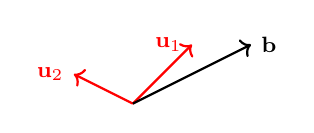
\begin{tikzpicture}[scale=0.75]
  \draw[red,thick,->] (0, 0) -- (1, 1) node[red, above, left]{{\footnotesize $\mf{u}_1$}};
  \draw[red,thick,->] (0, 0) -- (-1, 0.5) node[red, above, left]{{\footnotesize $\mf{u}_2$}};
  \draw[black,thick,->] (0, 0) -- (2, 1) node[black, above, right]{{\footnotesize $\mf{b}$}};
\end{tikzpicture}
\end{minipage}
\begin{minipage}{.3\textwidth}
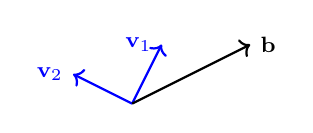
\begin{tikzpicture}[scale=0.75]
  \draw[blue,thick,->] (0, 0) -- (0.5, 1) node[blue, above, left]{{\footnotesize $\mf{v}_1$}};
  \draw[blue,thick,->] (0, 0) -- (-1, 0.5) node[blue, above, left]{{\footnotesize $\mf{v}_2$}};
  \draw[black,thick,->] (0, 0) -- (2, 1) node[black, above, right]{{\footnotesize $\mf{b}$}};
\end{tikzpicture}
\end{minipage}
\begin{minipage}{.3\textwidth}
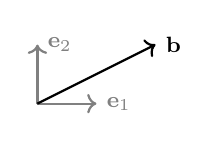
\begin{tikzpicture}[scale=0.75]
  \draw[gray,thick,->] (0, 0) -- (1, 0) node[gray, above, right]{{\footnotesize $\mf{e}_1$}};
  \draw[gray,thick,->] (0, 0) -- (0, 1) node[gray, above, right]{{\footnotesize $\mf{e}_2$}};
  \draw[black,thick,->] (0, 0) -- (2, 1) node[black, above, right]{{\footnotesize $\mf{b}$}};
\end{tikzpicture}
\end{minipage}
\end{center}
$\left\{\mf{v}_1, \mf{v}_2\right\}$, $\left\{\mf{u}_1, \mf{u}_2\right\}$ and $\left\{\mf{e}_1, \mf{e}_2\right\}$ are valid basis for $\mb{R}^2$, and the presentation for $\mf{b}$ in each one of them is different.

\item Finding out $\mf{a}$ is easiest when we are dealing with an orthonormal basis $\mf{U}$, in which case $\mf{a}$ is given by,
\[ \mf{a} = \begin{bmatrix*}\mf{u}_1^Tb\\ \mf{u}_2^Tb \\ \vdots \\ \mf{u}_n^Tb\end{bmatrix*} = \mf{U}^T\mf{b} = \mf{b}_{U} \]
\end{itemize}
\end{small}
\end{frame}


\begin{frame}[t]{Representation of vectors in a basis}
\demoex{1}{
  Consider a vector $\mf{b}$ whose representation in the standard basis is $\mf{b} = \begin{bmatrix*}2\\1\end{bmatrix*}$.

  $\bullet$ Consider a basis $V = \lc \begin{bmatrix*}[r]\sfrac{1}{\sqrt{5}}\\\sfrac{2}{\sqrt{5}}\end{bmatrix*}, \begin{bmatrix*}[r]-\sfrac{2}{\sqrt{5}}\\\sfrac{1}{\sqrt{5}}\end{bmatrix*} \rc$. Find out $\mf{b}_V$.
}\vspace{0.2cm}

\demoex{2}{
  $\bullet$ $ U = \lc \begin{bmatrix*}[r]1\\\frac{1}{2}\end{bmatrix*}, \begin{bmatrix*}[r]-\frac{1}{2}\\1\end{bmatrix*} \rc$. Find out $\mf{b}_U$.
}\vspace{0.2cm}

\demoex{3}{
  $\bullet$ $W = \lc \begin{bmatrix*}[r]1\\1\end{bmatrix*}, \begin{bmatrix*}[r]-1\\\frac{1}{2}\end{bmatrix*} \rc$. Find out $\mf{b}_W$.
}
\end{frame}


\begin{frame}[t]{Matrix Inverse}
\vspace{-0.25cm}
\begin{small}
\begin{itemize}
    \item Consider the equation $\mf{Ax} = \mf{y}$, where $\mf{A} \in \mb{R}^{n \times n}$ and $\mf{x}, \mf{y} \in \mb{R}^n$. 

    \item Let us assume $\mf{A}$ is non-singular $\implies$ columns of $\mf{A}$ represent a basis for $\mb{R}^n$.

    \item What does $\mf{x}$ represent? It is the representation of $\mf{y}$ in the basis consisitng of the columns of $\mf{A}$.
    \[ \mf{y} = \mf{Ax} = \begin{bmatrix*}\mf{a}_1 & \mf{a}_2 & \ldots & \mf{a}_n\end{bmatrix*}\begin{bmatrix*}x_1 \\ x_2 \\ \vdots \\ x_n\end{bmatrix*} = \sum_{i=1}^{n}\mf{a}_i x_i  \,\, \implies \,\, \mf{x} = \mf{A}^{-1}\mf{y} = \begin{bmatrix*}\tilde{\mf{b}}_1^T \\ \tilde{\mf{b}}_2^T \\ \ldots \\ \tilde{\mf{b}}_n^T\end{bmatrix*}\mf{y} = \begin{bmatrix*}\tilde{\mf{b}}_1^T\mf{y} \\ \tilde{\mf{b}}_2^T\mf{y} \\ \ldots \\ \tilde{\mf{b}}_n^T\mf{y}\end{bmatrix*} \]
    \item $\mf{A}^{-1}$ is a matrix that allows change of basis to the columns of $\mf{A}$ from the standard basis!
\end{itemize}
\end{small}

\demoex{2}{
\begin{footnotesize}
    $\bullet$ $W = \lc \begin{bmatrix*}[r]1\\1\end{bmatrix*}, \begin{bmatrix*}[r]-1\\\frac{1}{2}\end{bmatrix*} \rc$. Find $\mf{b}_W$ by calculating the inverse of the matrix $\mf{W} = \begin{bmatrix*}[r]1 & -1\\1 & \frac{1}{2}\end{bmatrix*}$. Does your answer match that of the previous approach? \vspace{0.2cm}

    $\bullet$ What about $V = \lc \begin{bmatrix*}[r]\sfrac{1}{\sqrt{5}}\\\sfrac{2}{\sqrt{5}}\end{bmatrix*}, \begin{bmatrix*}[r]-\sfrac{2}{\sqrt{5}}\\\sfrac{1}{\sqrt{5}}\end{bmatrix*} \rc$. What is $\mf{b}_V$?
\end{footnotesize}
}
\end{frame}


\begin{frame}[t]{Matrix Inverse}
\vspace{-0.25cm}
\begin{columns}
\begin{column}{0.5\textwidth}
\vspace{-0.2cm}
\begin{center}
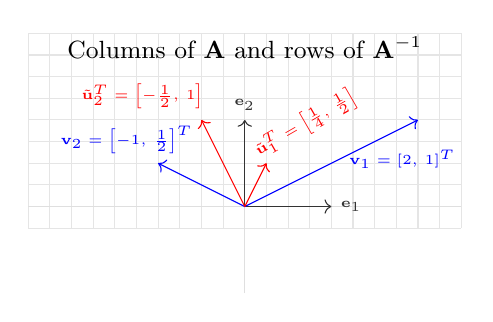
\begin{tikzpicture}[scale=1.1]
    % xy grid
    \draw[step=0.25, gray!20!, thin, xshift=0cm, yshift=0cm] (-2.5,-0.25) grid (2.5,2);
    \draw[gray!25!,thin] (-2.5,0) -- (2.5,0);
    \draw[gray!25!,thin] (0,-1) -- (0,2);
    \draw[black!80!, thin, ->] (0,0) -- (1,0) node[black!80!, right] {{\tiny $\mf{e}_1$}};
    \draw[black!80!, thin, ->] (0,0) -- (0,1) node[black!80!, above] {{\tiny $\mf{e}_2$}};
    \draw[blue, thin, ->] (0,0) -- (2, 1) node[xshift=-0.2cm, yshift=-0.5cm] {{\tiny $\mf{v}_1 = \left[2,\,1\right]^T$}};
    \draw[blue, thin, ->] (0,0) -- (-1, 1/2) node[xshift=-0.4cm, yshift=0.3cm] {{\tiny $\mf{v}_2 = \left[-1,\,\frac{1}{2}\right]^T$}};
    \draw[red, thin, ->] (0,0) -- (1/4, 1/2) node[xshift=0.5cm,yshift=0.5cm] {\rotatebox{30}{\tiny $\tilde{\mf{u}}_1^T = \left[\frac{1}{4},\,\frac{1}{2}\right]$}};
    \draw[red, thin, ->] (0,0) -- (-1/2, 1) node[xshift=-0.75cm, yshift=0.3cm] {{\tiny $\tilde{\mf{u}}_2^T = \left[-\frac{1}{2},\,1\right]$}};
    \node[above] at (0,1.6) {{\small Columns of $\mf{A}$ and rows of $\mf{A}^{-1}$}};
\end{tikzpicture}

\vspace{-0.5cm}
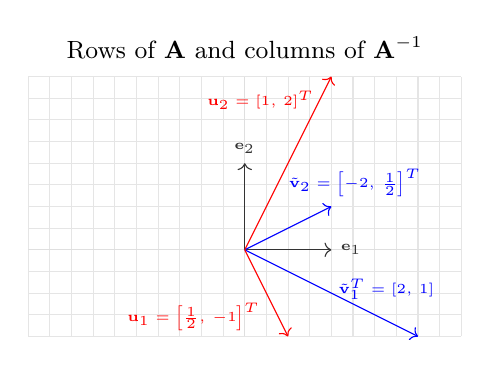
\begin{tikzpicture}[scale=1.1]
    % xy grid
    \draw[step=0.25, gray!20!, thin, xshift=0cm, yshift=0cm] (-2.5,-1) grid (2.5,2);
    \draw[gray!25!,thin] (-2.5,0) -- (2.5,0);
    \draw[gray!25!,thin] (0,-1) -- (0,2);
    \draw[black!80!, thin, ->] (0,0) -- (1,0) node[black!80!, right] {{\tiny $\mf{e}_1$}};
    \draw[black!80!, thin, ->] (0,0) -- (0,1) node[black!80!, above] {{\tiny $\mf{e}_2$}};
    \draw[blue, thin, ->] (0,0) -- (2, -1) node[xshift=-0.4cm, yshift=0.6cm] {{\tiny $\tilde{\mf{v}}_1^T = \left[2,\,1\right]$}};
    \draw[blue, thin, ->] (0,0) -- (1, 1/2) node[xshift=0.3cm, yshift=0.3cm] {{\tiny $\tilde{\mf{v}}_2 = \left[-2,\,\frac{1}{2}\right]^T$}};
    \draw[red, thin, ->] (0,0) -- (1/2, -1) node[xshift=-1.2cm,yshift=0.25cm] {{\tiny $\mf{u}_1 = \left[\frac{1}{2},\,-1\right]^T$}};
    \draw[red, thin, ->] (0,0) -- (1, 2) node[xshift=-0.9cm, yshift=-0.3cm] {{\tiny $\mf{u}_2 = \left[1,\,2\right]^T$}};
    \node[above] at (0,2.1) {{\small Rows of $\mf{A}$ and columns of $\mf{A}^{-1}$}};
\end{tikzpicture}
\end{center}
\end{column}

\begin{column}{0.5\textwidth}
\[ \mf{V} = \begin{bmatrix*}\mf{v}_1 & \mf{v}_2\end{bmatrix*} = \begin{bmatrix*}[r]2 & -1\\1 & \frac{1}{2}\end{bmatrix*}\]

\[ \mf{V}^{-1} = \begin{bmatrix*}\tilde{\mf{u}}_1^T \\ \tilde{\mf{u}}_2^T\end{bmatrix*} = \frac{1}{2}\begin{bmatrix*}[r]\frac{1}{2} & 1\\-1 & 2\end{bmatrix*}\]

\[ \mf{v}_1^T\tilde{\mf{u}}_1 = \mf{v}_2^T\tilde{\mf{u}}_2 = \tilde{\mf{v}}_1^T\mf{u}_1 = \tilde{\mf{v}}_2^T\mf{u}_2 = 1 \]

\[ \mf{v}_1^T\tilde{\mf{u}}_2 = \mf{v}_2^T\tilde{\mf{u}}_1 = \tilde{\mf{v}}_1^T\mf{u}_2 = \tilde{\mf{v}}_2^T\mf{u}_1 = 0 \]

\vspace{0.25cm}
\demoex{2}{
Verify these for $\mf{W} = \begin{bmatrix*}[r]1 & -1\\1 & \frac{1}{2}\end{bmatrix*}$ and $\mf{V} = \begin{bmatrix*}[r]\sfrac{1}{\sqrt{5}} & -\sfrac{2}{\sqrt{5}}\\\sfrac{2}{\sqrt{5}} & \sfrac{1}{\sqrt{5}}\end{bmatrix*}$.
}

\end{column}
\end{columns}
\end{frame}


\begin{frame}[t]{Left Inverse}
\vspace{-0.25cm}
\begin{itemize}
    \item Consider a rectangular matrix $\mf{A} \in \mb{R}^{m \times n}$. There exists no inverse $\mf{A}^{-1}$ for this matrix.

    \item But, does there exist two matrices $\mf{B}, \mf{C} \in \mb{R}^{n \times m}$, such that,
    \[ \mf{CA} = \mf{I}_n \,\,\,\,\, \text{ and } \,\,\,\,\, \mf{AB} = \mf{I}_m \]

    \item Both cannot be true for a rectangular matrix, only one can be true when the matrix is full rank.

    \item A rectangular matrix can only have either a left or a right inverse.

\end{itemize}

\demoex{2}{
    Consider a matrix $\mf{A} = \begin{bmatrix*}[r]1 & -2\\2 & 1\\1 & 1\end{bmatrix*}$. Let $\mf{B}, \mf{C}  \in \mb{R}^{2 \times 3}$. Can you explain why only $\mf{CA} = \mf{I}_2$ can be true and not $\mf{AB} = \mf{I}_3$? Can you also explain why $\mf{C}$ is not unique?
}
\end{frame}


\begin{frame}[t]{Left Inverse}
\vspace{-0.25cm}
\begin{itemize}
    \item Any non-zero $\mf{a} \in \mb{R}^{n \times 1} $ is left invertible: $ \mf{ba} = 1, \,\,\, \mf{b} \in \mb{R}^{1 \times n}; \,\,\,\,\, \mf{b}^T = \frac{\mf{a}}{\left\lVert \mf{a}\right\rVert^2} + \alpha \mf{a}^{\perp} $

    \item This can be generalized to $\mf{A} \in \mb{R}^{m \times n}$, $m > n$.
    \[ \lp \mf{C} + \hat{\mf{C}} \rp \mf{A} = \mf{I}_m \,\,\, \text{where } \mf{C}, \hat{\mf{C}} \in \mb{R}^{n \times m},\,\,\,{ }\hat{\mf{C}}\mf{A} = \mf{0}\]

    \item Condition for left inverse of $\mf{A}$ to exist: \textit{Colmuns of $\mf{A}$ must be independent.} $\longrightarrow rank\left(\mf{A}\right) = n \longrightarrow \mf{Ax} = 0 \implies \mf{x} = 0$.

    \item $\mf{Ax = b}$ can be solved, if and only if $\mf{A}\lp\mf{C}\mf{b}\rp = \mf{b}$, where $\mf{CA} = \mf{I}_n$.
\end{itemize}
\vspace{0.2cm}

\begin{small}
\demoex{2}{
    $\bullet$ Let $\mf{A} = \begin{bmatrix*}[r]1 & -2\\2 & 1\\1 & 1\end{bmatrix*}$. Find a complete solution for the left inverse of $\mf{A}$ such that $\lp\mf{C} + \hat{\mf{C}}\rp = \mf{I}_n$.
}\vspace{0.2cm}

\demoex{3}{
    $\bullet$ Consider the system, $\mf{Ax} = \mf{b}$. $\mf{A} = \begin{bmatrix*}[r]1\\2\end{bmatrix*}$, $\mf{x} = \begin{bmatrix*}x\end{bmatrix*}$, and $\mf{b} = \begin{bmatrix*}2\\4\end{bmatrix*}$. Find $\mf{x}$.
}\vspace{0.2cm}

\demoex{4}{
    $\bullet$ What happens when $\mf{b} = \begin{bmatrix*}1\\3\end{bmatrix*}$. What is $\mf{x}$?
}
\end{small}
\end{frame}


\begin{frame}[t]{Right Inverse}
% \vspace{-0.25cm}
\begin{itemize}
    \item For $\mf{A} \in \mb{R}^{m \times n}$, $n > m$ with full rank, $\mf{AB} = \mf{I}_m \longrightarrow \mf{B} \text{ is the right inverse.}$

    \item Right inverse of $\mf{A}$ exists only if the rows of $\mf{A}$ are independent, i.e. $rank\left(\mf{A}\right) = m$ $\longrightarrow \mf{A}^T\mf{x} = \mf{0} \implies \mf{x} = \mf{0}$

    \item $\mf{Ax} = \mf{b}$ can be solved for any $\mf{b}$. $\mf{x} = \mf{Bb} \implies \mf{A}\left(\mf{Bb}\right) = \mf{b}$. 

    \item There are an infitnite number of $\mf{B}$s $\implies$ an infinite number of solutions $\mf{x}$.
\end{itemize}
\vspace{0.2cm}

\demoex{2}{
    $\bullet$ Let $\mf{A} = \begin{bmatrix*}[r]1 & -2 & 1\\2 & 1 & -1\end{bmatrix*}$. Find a complete solution for the right inverse of $\mf{A}$.
}\vspace{0.2cm}

\demoex{3}{
    $\bullet$ Solve $\mf{A}\mf{x} = \begin{bmatrix*}[r]1 \\ 1\end{bmatrix*}$. Compare the solutions from Gauss-Jordan method and the ones obtained using right-inverses.
}\vspace{0.2cm}

\demoex{4}{
$\bullet$ Let $\mf{AB} = \mf{I}_m$. What about the relationship between $\mf{A}^T$ and $\mf{B}^T$?
}
\end{frame}


% \begin{frame}[t]{Fundamental subspaces of left and right inverses}
% \begin{columns}
% \begin{column}{0.5\textwidth}
% \textbf{Left Inverse}
% \begin{itemize}
%     \item $\mf{A} \in \mb{R}^{m \times n}$, $rank\lp\mf{A}\rp = n$
    
%     \item Subspaces of $\mf{A}$:\\
%     $\begin{array}{cc}
%     \mc{C}\lp\mf{A}\rp \in \mb{R}^m \,\,\, & \mc{N}\lp\mf{A}^T\rp \in \mb{R}^m\\
%     \mc{C}\lp\mf{A}^T\rp = \mb{R}^n \,\,\, & \mc{N}\lp\mf{A}\rp = \lc\mf{0}\rc
%     \end{array}$
    
%     \item Let $\mf{C} \in \mb{R}^{n \times m}$ be the left inverse of $\mf{A}$, such that $\mf{C}\mf{A} = \mf{I}_n$. What is $rank\lp\mf{C}\rp$? 

%     \item What about the subspaces of the left inverse?\\
%     \begin{itemize}
%         \item $\mc{C}\lp\mf{C}\rp$ \anim{2}{blue}{$= \mc{C}\lp\mf{A}^T\rp = \mb{R}^n$} \vspace{0.1cm}
%         \item $\mc{N}\lp\mf{C}^T\rp$ \anim{3}{blue}{$= \mc{N}\lp\mf{A}\rp = \lc\mf{0}\rc$} \vspace{0.1cm}
%         \item $\mc{C}\lp\mf{C}^T\rp$ \anim{4}{blue}{$= \mc{C}\lp\mf{A}\rp \in \mb{R}^m$} \vspace{0.1cm}
%         \item $\mc{N}\lp\mf{C}\rp$ \anim{5}{blue}{$= \mc{N}\lp\mf{A}^T\rp \in \mb{R}^m$}
%     \end{itemize}
% \end{itemize}
% \end{column}
% \begin{column}{0.5\textwidth}
% \onslide<6->{
% \textbf{Right Inverse}
% \begin{itemize}
%     \item $\mf{A} \in \mb{R}^{m \times n}$, $rank\lp\mf{A}\rp = m$
    
%     \item Subspaces of $\mf{A}$:\\
%     $\begin{array}{cc}
%     \mc{C}\lp\mf{A}\rp = \mb{R}^m \,\,\, & \mc{N}\lp\mf{A}^T\rp = \lc\mf{0}\rc\\
%     \mc{C}\lp\mf{A}^T\rp \in \mb{R}^n \,\,\, & \mc{N}\lp\mf{A}\rp \in \mb{R}^n
%     \end{array}$
    
%     \item Let $\mf{B} \in \mb{R}^{n \times m}$ be the left inverse of $\mf{A}$, such that $\mf{A}\mf{B} = \mf{I}_m$. What is $rank\lp\mf{B}\rp$? 

%     \item What about the subspaces of the left inverse?\\
%     \begin{itemize}
%         \item $\mc{C}\lp\mf{B}\rp$ \anim{7}{blue}{$= \mc{C}\lp\mf{A}^T\rp \in \mb{R}^n$} \vspace{0.1cm}
%         \item $\mc{N}\lp\mf{B}^T\rp$ \anim{8}{blue}{$= \mc{N}\lp\mf{A}\rp \in \mb{R}^n$} \vspace{0.1cm}
%         \item $\mc{C}\lp\mf{B}^T\rp$ \anim{9}{blue}{$= \mc{C}\lp\mf{A}\rp = \mb{R}^m$} \vspace{0.1cm}
%         \item $\mc{N}\lp\mf{B}\rp$ \anim{10}{blue}{$= \mc{N}\lp\mf{A}^T\rp = \lc\mf{0}\rc$}
%     \end{itemize}
% \end{itemize}}
% \end{column}
% \end{columns}
% \end{frame}


\begin{frame}[t]{Pseudo Inverse}
% \vspace{-0.25cm}
\begin{itemize}
    \item Consider a tall, skinny  matrix $\mf{A} \in \mb{R}^{m \times n}$ with independent columns. It turns out the Gram matrix $\mf{A}^T\mf{A} \in \mb{R}^{n \times n}$ is invertible. If that is the case then,
    \[ \left(\mf{A}^T\mf{A}\right)^{-1}\mf{A}^T\mf{A} = \mf{I}_n; \,\,\,\,\, \left(\mf{A}^T\mf{A}\right)^{-1}\mf{A}^T \text{ is a left inverse.} \]
    \item $\mf{A}^{\dagger} = \left(\mf{A}^T\mf{A}\right)^{-1}\mf{A}^T$ is called the \textit{pseudo inverse} or the \textit{Moore-Penrose inverse}.

    \item For the case of a fat, wide matrix, we have $\mf{A}^{\dagger} = \mf{A}^T\left(\mf{AA}^T\right)^{-1}$.

    \item When $\mf{A}$ is square and invertible, $\mf{A}^{\dagger} = \mf{A}^{-1}$.
\end{itemize}
\vspace{0.2cm}

\demoex{2}{
    $\bullet$ Solve $\mf{Ax} = \mf{b}$ using the $\mf{A}^\dagger$. $\mf{A} = \begin{bmatrix*}[r]1\\2\end{bmatrix*}$, and $\mf{b} = \begin{bmatrix*}2\\4\end{bmatrix*}$. Find $\mf{x}$.
}\vspace{0.2cm}

\demoex{3}{
    $\bullet$ Compare $\mf{A}^\dagger$ with that of the general left inverse $\mf{C}$. Calculate $\lV \mf{C} \rV^2$ and find out the $\min \lV\mf{C}\rV^2$. What is $\lV\mf{A}^\dagger\rV^2$?
}\vspace{0.2cm}
\end{frame}


\begin{frame}[t]{Matrix Inverse and Pseudo Inverse through $\mf{QR}$ factorization}
\begin{itemize}
    \item Consider an invertible, square matrix $\mf{A} \in \mb{R}^{n \times n}$. 
    \[ \mf{A} = \mf{QR} \implies \mf{A}^{-1} = \left(\mf{QR}\right)^{-1} = \mf{R}^{-1}\mf{Q}^{-1} = \mf{R}^{-1}\mf{Q}^T \] 
    where, $\mf{R}, \mf{Q} \in \mb{R}^{n \times n}$. $\mf{R}$ is upper triangular, and $\mf{Q}$ is an orthogonal matrix.
    
    \item In the case of a left invertible rectangular matrix $\mf{A} \in \mb{R}^{m \times n}$, we can factorize $\mf{A} = \mf{QR}$, with $\mf{Q} \in \mb{R}^{m \times n}$ and $\mf{R} \in \mb{R}^{m \times m}$.
    \[ \mf{A}^{\dagger} = \left(\mf{A}^T\mf{A}\right)^{-1}\mf{A}^T = \left(\mf{R}^T\mf{Q}^T\mf{QR}\right)^{-1}\mf{R}^T\mf{Q}^T = \left(\mf{R}^T\mf{R}\right)^{-1}\mf{R}^T\mf{Q}^T = \mf{R}^{-1}\mf{Q}^T \]
    
    \item For a right invertible wide, fat matrix, we can find out the pseudo-inverse of $\mf{A}^T$, and then take the transpose of the pseudo-inverse.
    \[ \mf{AA}^{\dagger} = \mf{I} \implies \left(\mf{A}^{\dagger}\right)^T\mf{A}^T = \left(\mf{A}^T\right)^{\dagger}\mf{A}^T = \mf{I} \]
    \[ \mf{A}^T = \mf{QR} \implies \left(\mf{A}^T\right)^{\dagger} = \mf{R}^{-1}\mf{Q}^T = \left(\mf{A}^{\dagger}\right)^T \implies  \mf{A}^{\dagger} = \mf{QR}^{-T} \]
\end{itemize}
\end{frame}

\end{document}